%%%%%%%%%%%%%%%%%%%%%%%%%%%%%%%%%%%%%%%%%
% University/School Laboratory Report
% LaTeX Template
% Version 3.1 (25/3/14)
%
% This template has been downloaded from:
% http://www.LaTeXTemplates.com
%
% Original author:
% Linux and Unix Users Group at Virginia Tech Wiki 
% (https://vtluug.org/wiki/Example_LaTeX_chem_lab_report)
%
% License:
% CC BY-NC-SA 3.0 (http://creativecommons.org/licenses/by-nc-sa/3.0/)
%
%%%%%%%%%%%%%%%%%%%%%%%%%%%%%%%%%%%%%%%%%

%----------------------------------------------------------------------------------------
%	PACKAGES AND DOCUMENT CONFIGURATIONS
%----------------------------------------------------------------------------------------

\documentclass{article}

\usepackage[version=3]{mhchem} % Package for chemical equation typesetting
\usepackage{siunitx} % Provides the \SI{}{} and \si{} command for typesetting SI units
\usepackage{graphicx} % Required for the inclusion of images
\usepackage{natbib} % Required to change bibliography style to APA
\usepackage{amsmath} % Required for some math elements 
\usepackage{indentfirst}
\usepackage{float}
\usepackage{booktabs}
\usepackage{enumerate}
\usepackage{url}
\usepackage[final]{pdfpages}
\usepackage{geometry}
\usepackage{pgfgantt}
\usepackage{graphicx}
\geometry{left = 2cm, right = 2cm, top = 0.5cm, bottom = 2cm}



\renewcommand{\labelenumi}{\alph{enumi}.} % Make numbering in the enumerate environment by letter rather than number (e.g. section 6)

%\usepackage{times} % Uncomment to use the Times New Roman font

%----------------------------------------------------------------------------------------
%	DOCUMENT INFORMATION
%----------------------------------------------------------------------------------------

\title{STATS 506 Project Report} % Title
\author{Zicong Xiao, Yulin Gao, Qianang Chen, Xiaoyang Sheng}

\begin{document}


\maketitle % Insert the title, author and date



% If you wish to include an abstract, uncomment the lines below
% \begin{abstract}
% Abstract text
% \end{abstract}

%----------------------------------------------------------------------------------------
%	SECTION 1
%----------------------------------------------------------------------------------------

\section{Introduction}
\subsection{Topic}
An urban heat island (UHI) is an urban area which becomes islands of higher temperatures relative to the surrounding rural areas. This phenomenon is caused by human activity, materials of infrastructures, climate change and etc. It will cause residents some severe diseases like asthma and stroke, especailly to population who are over 65 years old. Yet the government can adopt some measures, for example, increase the insurance rates and medical expenditure to mitigate the harmful effects. We looked into data from mainly two sources: First we collected the climate data from earth engine, with covariates like surface temperature and percipitation, which are significant factors in our model. On the other hand we extracted the health data from CDC and chose the variables like mortality of different age groups, insurance rates and prevalence of asthma. Then we'll use different models (linear regression, Bayesian hierarchical model, random forest) to make vulnerability assessment towards the health of older adults. Next we'll do some model checking and validation to evaluate the model fitness. Finally based on the results we obtained, we'll do some analysis on negative impact of UHI on public health, along with the effect of each covariate.
\section{Investigation Plan}
\subsection{Data set}
\begin{itemize}
    \item United States Surface Urban Heat Island database; from Mendeley Data: \url{https://data.mendeley.com/datasets/x9mv4krnm2/2}
    \item Global map temperature; from NASA: \url{https://giovanni.gsfc.nasa.gov/giovanni/#service=TmAvMp&starttime=&endtime=&variableFacets=dataFieldMeasurement%3ASurface%20Temperature%3B&dataKeyword=AIRS3STM}
    \item Death of elderly people by county from CDC: \url{https://wonder.cdc.gov/ucd-icd10.html}
    \item Insurance rate of each US county from US Census: \url{http://data.ctdata.org/dataset/health-insurance-coverage}
\end{itemize}

\section{Bayesian Linear Model}
\subsection{Model Selection}
In this section we build the Bayesian linear model with respect to the prevalence of stroke and UHI/climate effects, and the insurance rate is also taken into account. Let $y_i(i=1,2,...,N)$ be the mean of people who had got stroke within a county in three years(2017-2019), $N=427$ is the number of counties we choose. We define $x_1$ as the UHI index in summer during the day, $x_2$ as the UHI index in summer at night, $x_3$ as the mean air temperature and $x_4$ as the insurance rate within a county. The likelihood distribution is defined as follows:
\begin{equation}\label{d}
        y_i \overset{\mathrm{iid}}{\sim} N(\mu_i,\sigma_2)
\end{equation}
\begin{equation}\label{d}
	\mu_i=\beta_0+\beta_1x_1+\beta_2x_2+\beta_3x_3+\beta_4x_4
\end{equation}
Then we define the noninformative priors of parameters as follows:
\begin{equation}
	\begin{aligned}
		\beta_i\sim U(-1\mathrm{e}6,1\mathrm{e}6),i=0,1,2,3,4
		\\
		\sigma^{-2}\sim \mathrm{G}(-1\mathrm{e}6,1\mathrm{e}6)
	\end{aligned}
\end{equation}
\subsection{Fitting and Results}
We use flat priors, 5 chains, 100K iterations and 50K burn-in periods in our MCMC simulation. The posteriors of each parameter of population over 65 and under 65 are as follows:
\\
\begin{center}
\begin{tabular}{l*{5}{c}r}
	Parameter             & mean(over 65) &95\% CI(over 65) & mean(under 65) & 95\% CI(under 65) \\
	\hline
	$\beta_0$          & -261.758 & (-803.703,173.850)  & -168.118 & (-219.075,-99.355)  \\
	$\beta_1$            & 5.135 & (-0.028,10.241) & 1.258 & (0.595,1.920) \\
	$\beta_2$            & 1.956 & (-10.971,15.151) & 1.010 & (-0.630,2.643)\\
	$\beta_3$           & 1.960 & (0.772,3.502)  & 0.703 & (0.517,0.840) \\
	$\beta_4$           & -0.557 & (-1.899,0.884)& -0.174 & (-0.360,0.001)  \\
\end{tabular}
\end{center}

\subsection{Analysis and Discussion}
From the tables above we find that the effect of UHI index is more significant than mean air temperature and the prevalence of stroke in all age groups will grow with the increase of UHI index and mean air temperature. 
\\
\indent
We also find that although $\beta_2$ is positive, but the 95\% credible intervals both contain 0. Use R, the probabilities that $\beta_2>0$ from each group are 0.6136 and 0.8854, so we can conclude that the UHI index in summer at night has weaker effect to public health than the other two covariates. The UHI effect is stronger at night based on scientific literatures, which means the index tend to be higher. But the temperature at night is also lower, so people aren't as vulnerable to heat-related illness, which causes $\beta_2<\beta_1$.
\\
\indent
The mean value of $\beta_4$ is negative in both tables. If the rate of insurance coverage within a county is higher, which depends on government funding and people's awareness of health, then the residents will be less vulnerable to all kinds of diseases. 
\\
\indent
The first three parameters in table 1 are all greater than the corresponding parameters in table 2, so the variables of mean air temperatures and UHI index have a greater effect to older adults who are 65 years old. Since their immunities are going down, they are more susceptible to external factors than young adults. The parameter $\beta_4$ in table 1 is less than that in table 2, which implies that the insurance coverage guarantee more interests to older populations, and their diseases may be more treatable.
\\
\indent
We can improve the fitness of model by increasing the number of chains, burn-in periods and thinning rates, or considering the interaction between variables.
\section{Appendix}
\begin{figure}[H]
\centering
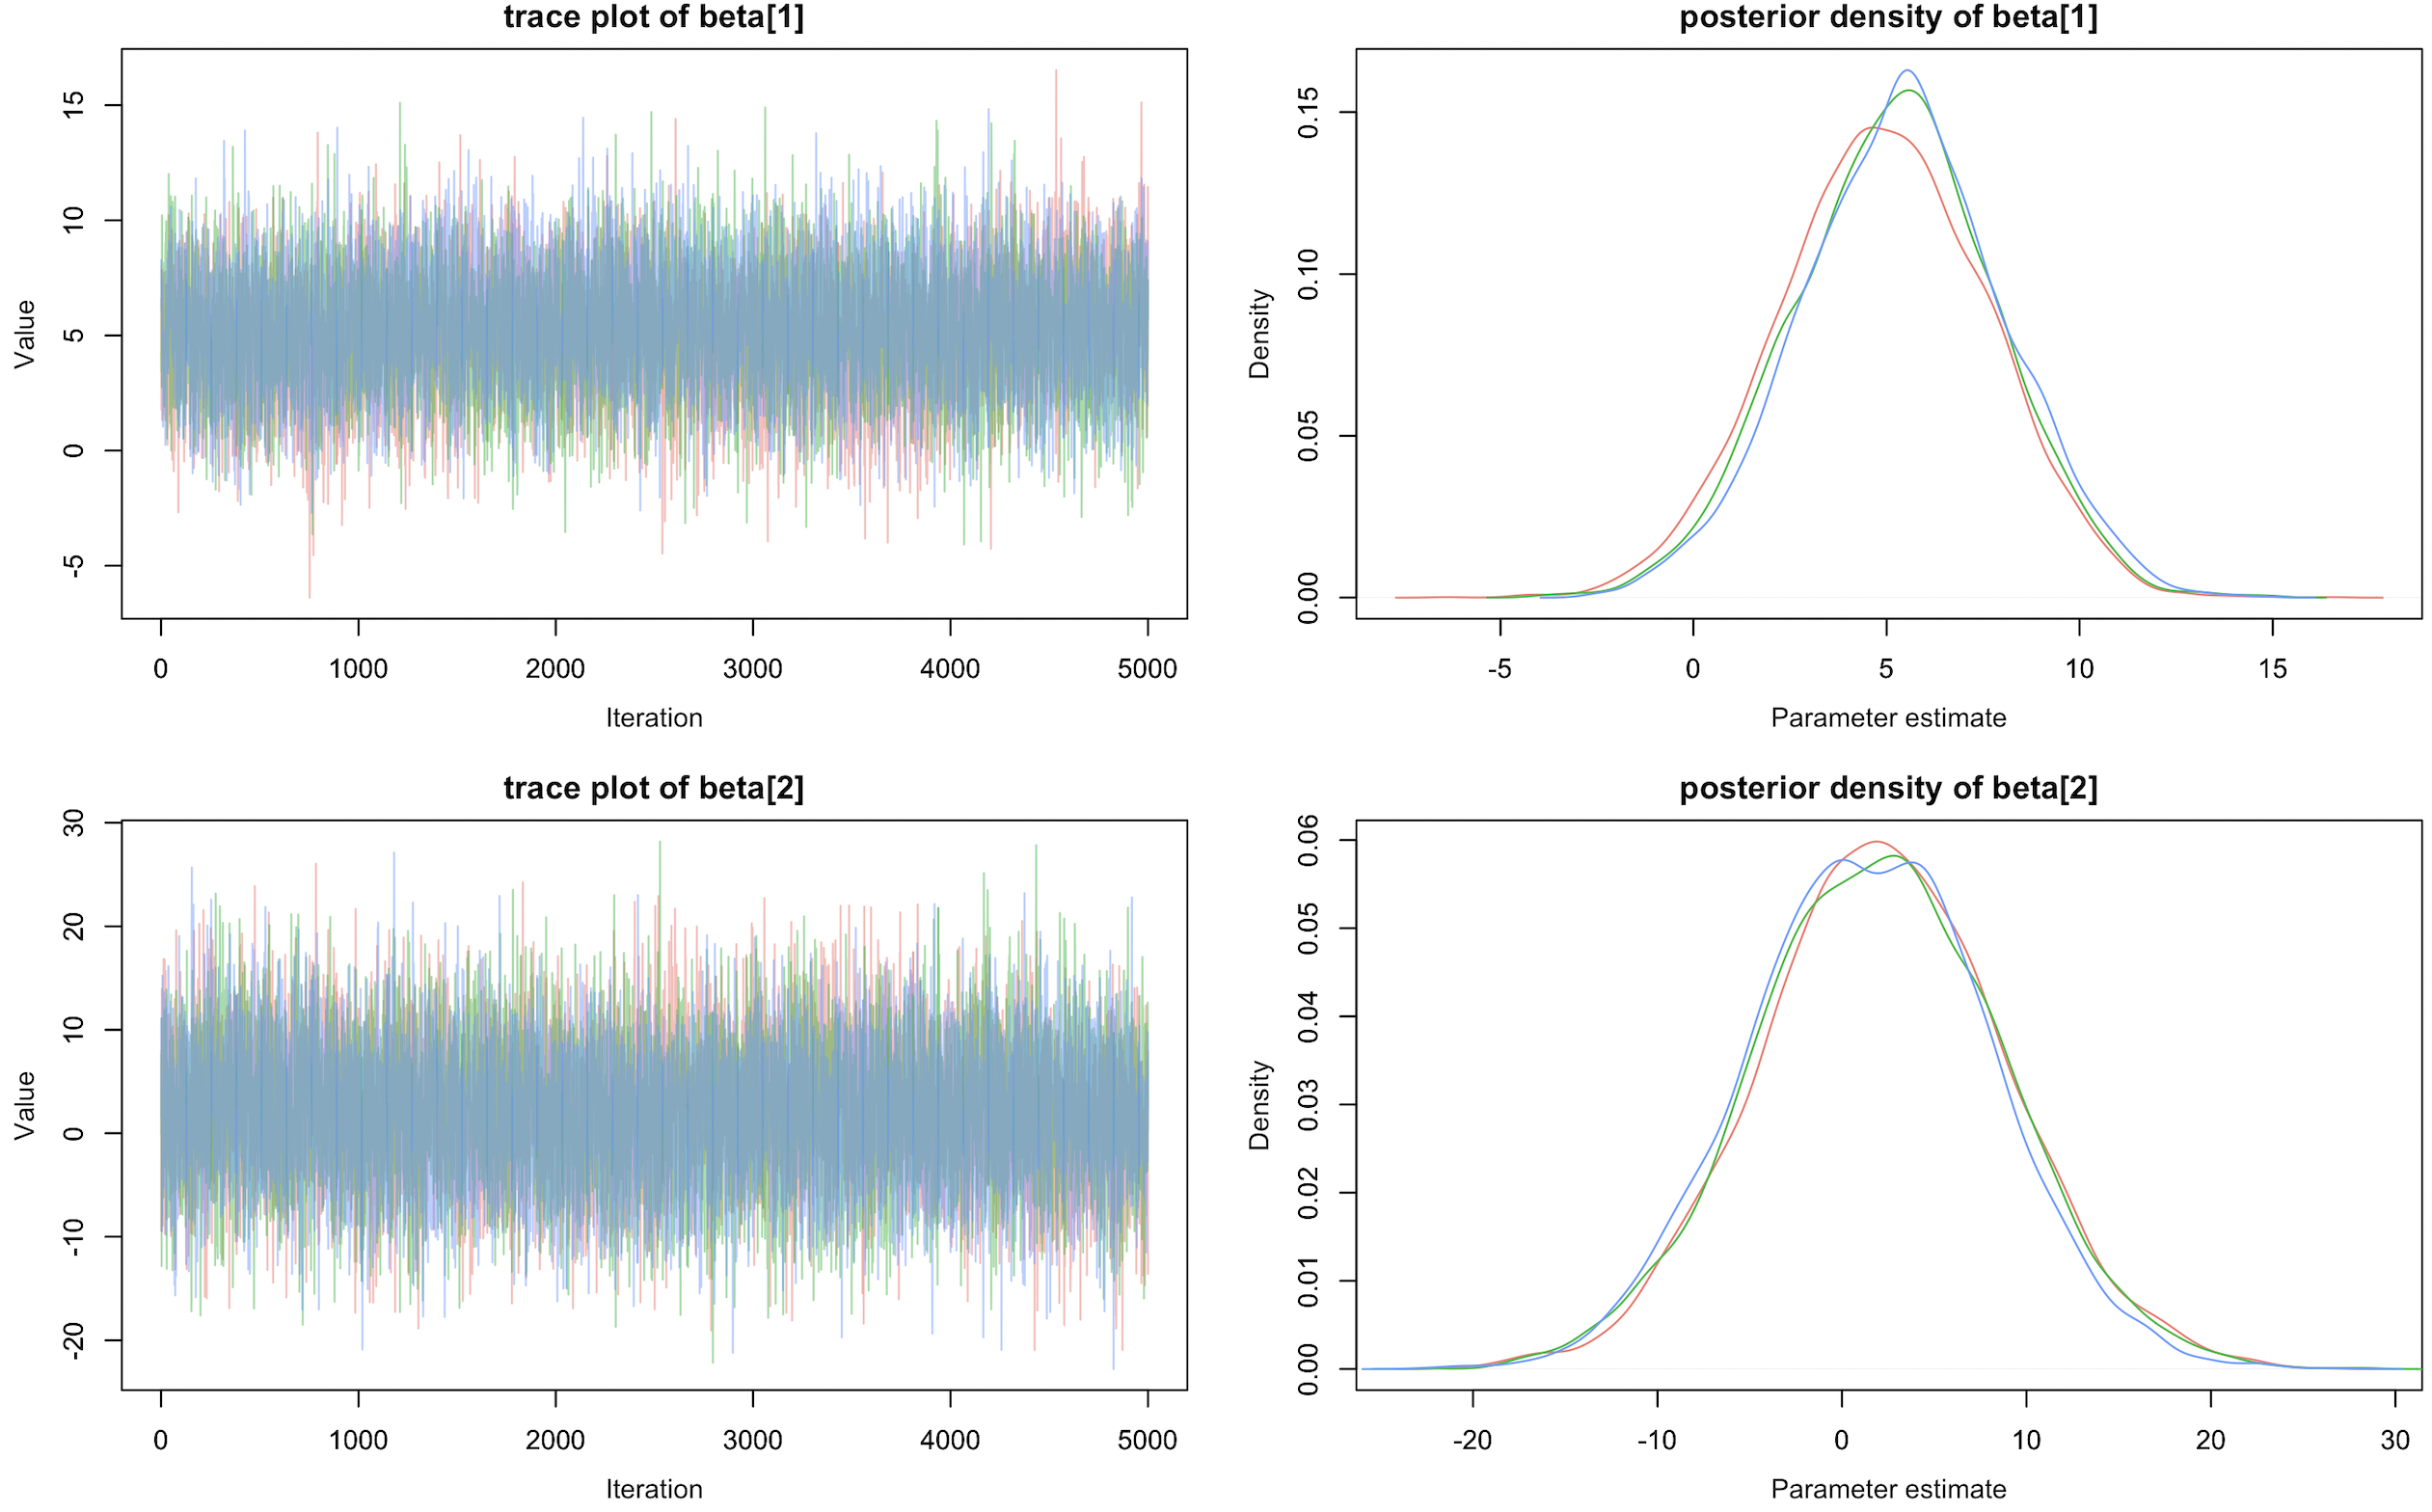
\includegraphics[scale=0.3]{plot1.png}
\caption{The trace plot and posterior pdf of $\beta_1$ and $\beta_2$ from the MCMC output of population over 65}
\end{figure}
\begin{figure}[H]
\centering
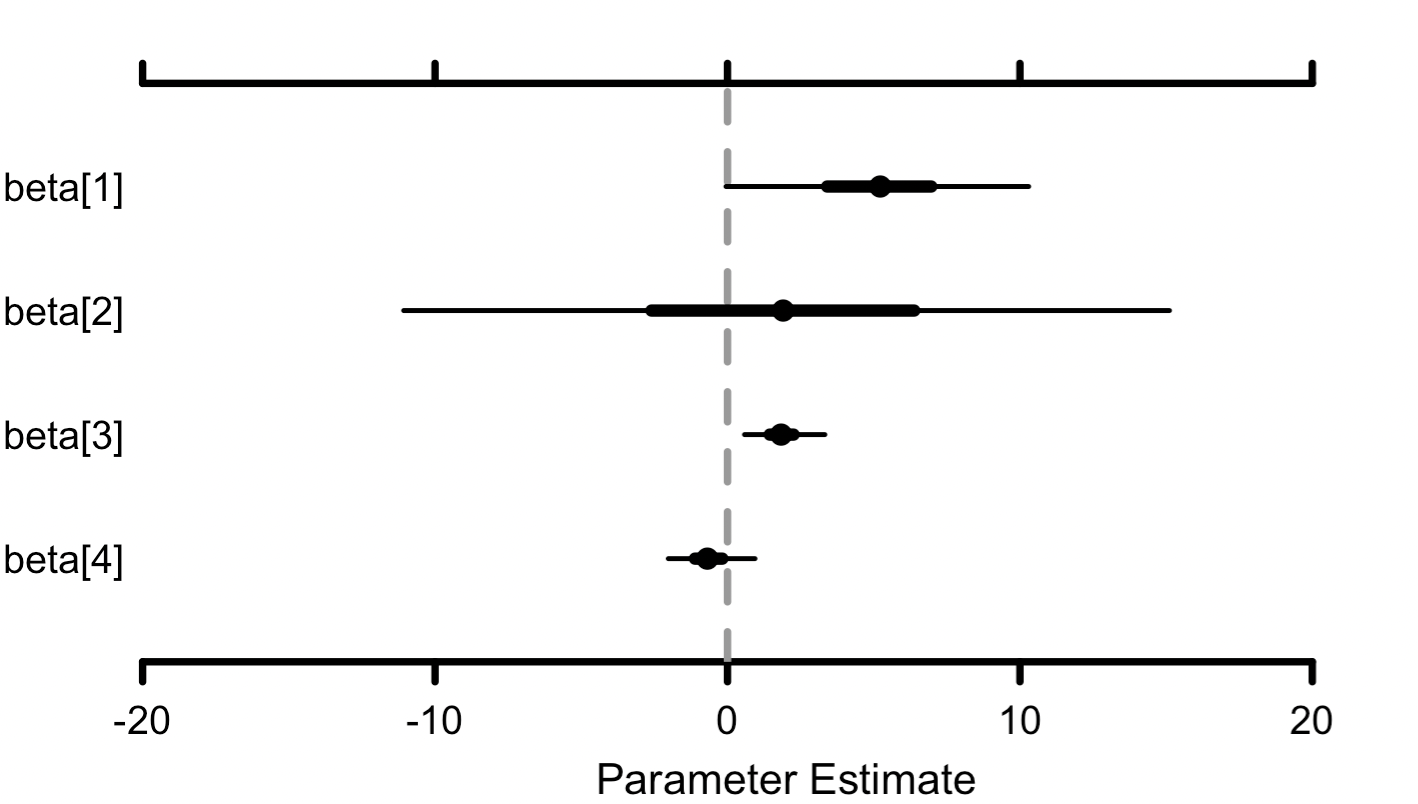
\includegraphics[scale=0.3]{beta1.png}
\caption{The caterpillar plot of $\beta_i$ from the output of population over 65}
\end{figure}
\begin{figure}[H]
\centering
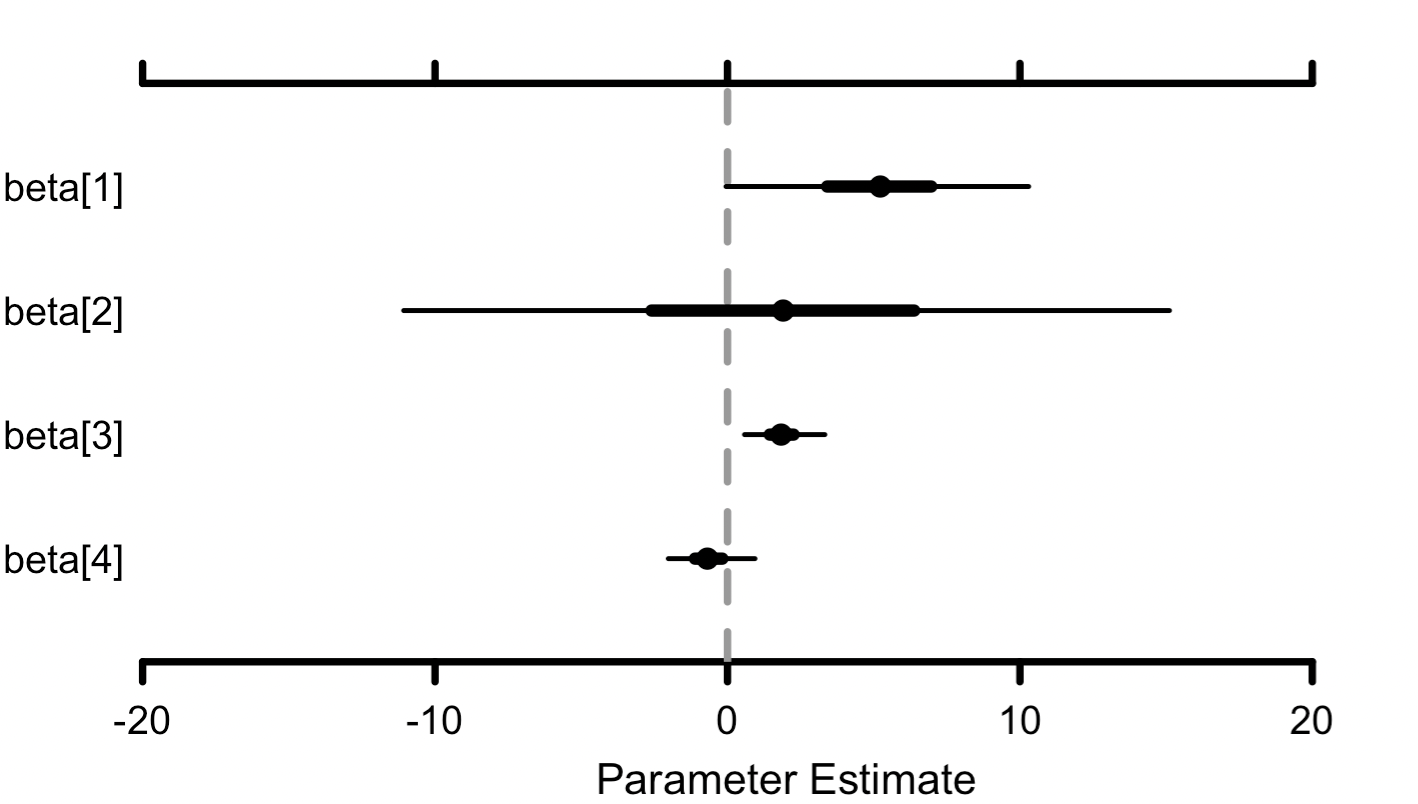
\includegraphics[scale=0.3]{beta1.png}
\caption{The caterpillar plot of $\beta_i$ from the output of population under 65}
\end{figure}
\end{document}